% Created 2016-03-27 日 20:12
\documentclass[xcolor=svgnames,presentation]{beamer}
\usepackage[utf8]{inputenc}
\usepackage[T1]{fontenc}
\usepackage{fixltx2e}
\usepackage{graphicx}
\usepackage{longtable}
\usepackage{float}
\usepackage{wrapfig}
\usepackage{soul}
\usepackage{textcomp}
\usepackage{marvosym}
\usepackage{wasysym}
\usepackage{latexsym}
\usepackage{amssymb}
\usepackage{hyperref}
\tolerance=1000
\usepackage{minted}
\usecolortheme[named=FireBrick]{structure}\setbeamercovered{transparent}\setbeamertemplate{caption}[numbered]\setbeamertemplate{blocks}[rounded][shadow=true] \usetheme{Darmstadt}\date{\today} \usepackage{tikz}\usepackage{xeCJK}\usepackage{amsmath}\setmainfont{Times New Roman}\setCJKmainfont[BoldFont={Adobe Heiti Std},ItalicFont={Adobe Fangsong Std}]{Adobe Heiti Std}\setCJKsansfont{Adobe Heiti Std}\setCJKmonofont{Adobe Fangsong Std}\usepackage{verbatim}\graphicspath{{figures/}} \definecolor{lstbgcolor}{rgb}{0.9,0.9,0.9} \usepackage{listings}\usepackage{minted} \usepackage{fancyvrb}\usepackage{xcolor}\lstset{escapeinside=`',frameround=ftft,language=C,breaklines=true,keywordstyle=\color{blue!70},commentstyle=\color{red!50!green!50!blue!50},frame=shadowbox,backgroundcolor=\color{yellow!20},rulesepcolor=\color{red!20!green!20!blue!20}}
\usemintedstyle{default}
\providecommand{\alert}[1]{\textbf{#1}}

\title{第4讲 Linux基础(3)}
\author{王晓庆}
\date{\today}
\hypersetup{
  pdfkeywords={},
  pdfsubject={},
  pdfcreator={Emacs Org-mode version 7.9.3f}}

\institute{wangxiaoqing@outlook.com}
\begin{document}

\maketitle

\begin{frame}
\frametitle{Outline}
\setcounter{tocdepth}{1}
\tableofcontents
\end{frame}

\section{正则表达式}
\label{sec-1}
\subsection{正则表达式}
\label{sec-1-1}
\begin{frame}
\frametitle{正则表达式}
\label{sec-1-1-1}
\begin{itemize}

\item 正则表达式由字符与元字符组成,整个表达式用于描述符合某些特定特征的一类字符串。
\label{sec-1-1-1-1}%

\item 最基本的正则表达式匹配单个字符,大多数字符都与其自身匹配,少数具有特殊含义的元字符可以在其前面加反斜杠进行引用。
\label{sec-1-1-1-2}%

\item Linux中许多工具都支持正则表达式,各种编程语言也包含了处理正则表达式的库。
\label{sec-1-1-1-3}%
\end{itemize} % ends low level
\end{frame}
\begin{frame}[fragile]
\frametitle{基本正则表达式(BRE)元字符}
\label{sec-1-1-2}
\begin{exampleblock}{. 表示单个任意字符}
\label{sec-1-1-2-1}


\begin{minted}[]{bash}
grep 'a.b' file
grep 'a\.b' file
\end{minted}
\end{exampleblock}
\begin{block}{[xyz] 表示单个括号中列出的字符}
\label{sec-1-1-2-2}


\begin{minted}[]{bash}
grep '[0-9]\.[0-9]' file
grep '[^0-9][0-9][^0-9]' file
\end{minted}
\end{block}
\begin{exampleblock}{x* 表示其左边的项x出现0次以上}
\label{sec-1-1-2-3}


\begin{minted}[]{bash}
grep '[0-9][0-9]*' file
\end{minted}
\end{exampleblock}
\end{frame}
\begin{frame}[fragile]
\frametitle{基本正则表达式(BRE)元字符}
\label{sec-1-1-3}
\begin{itemize}

\item 位置锚定
\label{sec-1-1-3-1}%
\end{itemize} % ends low level
\begin{exampleblock}{\^{} x 匹配位于行首的x}
\label{sec-1-1-3-2}


\begin{minted}[]{bash}
grep '^#' file
grep -v '^#' file
grep '^[^#]' file
\end{minted}
\end{exampleblock}
\begin{block}{y\$ 匹配位于行尾的y}
\label{sec-1-1-3-3}


\begin{minted}[]{bash}
grep '[0-9]$' file
grep -v '^$' file | wc -l
\end{minted}
\end{block}
\end{frame}
\begin{frame}
\frametitle{扩展正则表达式(ERE)元字符}
\label{sec-1-1-4}
\begin{itemize}

\item 扩展正则表达式元字符
\label{sec-1-1-4-1}%
\begin{itemize}

\item ? + | \{ \} ( )
\label{sec-1-1-4-1-1}%
\end{itemize} % ends low level

\item ERE元字符被视为普通字符,除非在其前面加上反斜杠!
\label{sec-1-1-4-2}%
\end{itemize} % ends low level
\end{frame}
\begin{frame}[fragile]
\frametitle{扩展正则表达式(ERE)元字符(2)}
\label{sec-1-1-5}
\begin{exampleblock}{x+ 表示其左边的项x出现1次以上}
\label{sec-1-1-5-1}


\begin{minted}[]{bash}
grep '[0-9]\+' file
grep -E '[0-9]+' file
egrep '[0-9]+' file
\end{minted}
\end{exampleblock}
\begin{block}{x? 表示其左边的项x出现0次或1次}
\label{sec-1-1-5-2}


\begin{minted}[]{bash}
grep '[0-9]*\.?[0-9]\+' file
\end{minted}
\end{block}
\begin{exampleblock}{x|y 表示x或y}
\label{sec-1-1-5-3}


\begin{minted}[]{bash}
grep 'html|HTML' file
\end{minted}
\end{exampleblock}
\end{frame}
\begin{frame}[fragile]
\frametitle{扩展正则表达式(ERE)元字符(3)}
\label{sec-1-1-6}
\begin{exampleblock}{x\{m\} 表示x出现m次}
\label{sec-1-1-6-1}


\begin{minted}[]{bash}
grep '\$[0-9]\{2\}\.[0-9]{\2\}[^0-9]' file
\end{minted}
\end{exampleblock}
\begin{block}{x\{m,\} 表示x出现m次以上}
\label{sec-1-1-6-2}


\begin{minted}[]{bash}
grep '\$[0-9]\{5,\}\.[0-9]{\2\}[^0-9]' file
\end{minted}
\end{block}
\begin{exampleblock}{x\{m,n\} 表示x出现m到n次(m<n)}
\label{sec-1-1-6-3}


\begin{minted}[]{bash}
grep '\$[0-9]\{3,4\}\.[0-9]{\2\}[^0-9]' file
\end{minted}
\end{exampleblock}
\end{frame}
\begin{frame}[fragile]
\frametitle{扩展正则表达式(ERE)元字符(4)}
\label{sec-1-1-7}
\begin{exampleblock}{()与\n 组合与反向引用}
\label{sec-1-1-7-1}


\begin{minted}[]{bash}
grep '\([0-9]\+\)\.\1' file
grep '^\(.\).*\1$' file
\end{minted}
\end{exampleblock}
\begin{block}{试一试}
\label{sec-1-1-7-2}

\begin{enumerate}
\item 如何在/usr/share/dict/words中查找长度为5的回文单词?
\item 如何滤出类似<em>warning</em>这样的行?
\item 如何查找包含相邻重复词的行?
\end{enumerate}
\end{block}
\note{答案


\begin{minted}[]{bash}
egrep '(.)(.).\2\1' /usr/share/dict/words #长度为5的回文词
egrep '<([^>]*)>[^<]*</\1>' index.html    #一对html标记
grep '\<\([a-zA-Z]\+\)\> \1' learn-vim    #相邻重复单词
\end{minted}
}
\end{frame}
\begin{frame}[fragile]
\frametitle{字符类}
\label{sec-1-1-8}
\begin{itemize}

\item 为应更多语言环境,POSIX定义了若干字符类\\
\label{sec-1-1-8-1}%
\begin{verbatim}
[:alnum:] 数字、字母
[:alpha:] 字母
[:blank:] 空格符、制表符
[:cntrl:] 控制字符
[:digit:] 数字0-9
[:graph:] 数字、字母、标点符号
[:lower:] 小写字母
[:print:] 数字、字母、标点符号、空格符
[:punct:] 标点符号
[:space:] 制表符、换行符、回车符、空格符
[:upper:] 大写字母
[:xdigit:] 十六进制数字0-9a-fA-F
\end{verbatim}
\end{itemize} % ends low level
\end{frame}
\begin{frame}[fragile]
\frametitle{反斜杠字符}
\label{sec-1-1-9}
\begin{itemize}

\item 有些字符前加上反斜杠后具有特殊含义\\
\label{sec-1-1-9-1}%
\begin{verbatim}
\b 匹配单词边缘的空字符串
\B 匹配非单词边缘的空字符串
\< 匹配单词开头的空字符串
\> 匹配单词结尾的空字符串
\w 匹配单词字符,即[_[:alnum:]]
\W 匹配非单词字符,即[^_[:alnum:]]
\s 匹配空白符,即[[:space:]]
\S 匹配非空白符,即[^[:space:]]
\end{verbatim}
\end{itemize} % ends low level
\end{frame}
\begin{frame}[fragile]
\frametitle{字符类和反斜杠字符举例}
\label{sec-1-1-10}
\begin{exampleblock}{字符类示例}
\label{sec-1-1-10-1}


\begin{minted}[]{bash}
tr -d '[:punct:]' <file
grep '[[:digit:]]\+$' file #注意两层中括号的区别
\end{minted}
\end{exampleblock}
\begin{block}{反斜杠字符示例}
\label{sec-1-1-10-2}


\begin{minted}[]{bash}
grep \bconfident\b /usr/share/dict/words
grep \Bconfident\B /usr/share/dict/words
\end{minted}
\end{block}
\end{frame}
\begin{frame}[fragile]
\frametitle{fgrep(fixed fgrep)}
\label{sec-1-1-11}
\begin{itemize}

\item 等同于grep -F
\label{sec-1-1-11-1}%

\item fgrep将所有字符都看作普通字符,搜索速度快!
\label{sec-1-1-11-2}%

\item fgrep可以同时搜索以换行符隔开的多个字符串
\label{sec-1-1-11-3}%
\end{itemize} % ends low level
\begin{exampleblock}{示例}
\label{sec-1-1-11-4}


\begin{minted}[]{bash}
fgrep 'normal mode
insert mode
command-line mode' learn-vim
\end{minted}
\end{exampleblock}
\end{frame}
\begin{frame}[fragile]
\frametitle{在find命令中使用正则表达式}
\label{sec-1-1-12}
\begin{itemize}

\item -regex 匹配正则表达式
\label{sec-1-1-12-1}%

\item -iregex 同上且忽略大小写
\label{sec-1-1-12-2}%
\end{itemize} % ends low level
\begin{exampleblock}{示例}
\label{sec-1-1-12-3}


\begin{minted}[]{bash}
find /usr/bin -regex 'mk'     #:-(
find /usr/bin -regex '.*mk.*' #:-)
\end{minted}
\end{exampleblock}
\end{frame}
\section{sed和awk}
\label{sec-2}
\subsection{sed}
\label{sec-2-1}
\begin{frame}
\frametitle{sed简介}
\label{sec-2-1-1}
\begin{itemize}

\item sed(stream editor)\\
\label{sec-2-1-1-1}%
sed提供非交互式批量文本编辑功能,例如在100个文件中,处理20个不同的编辑操作。

\item sed的工作原理\\
\label{sec-2-1-1-2}%
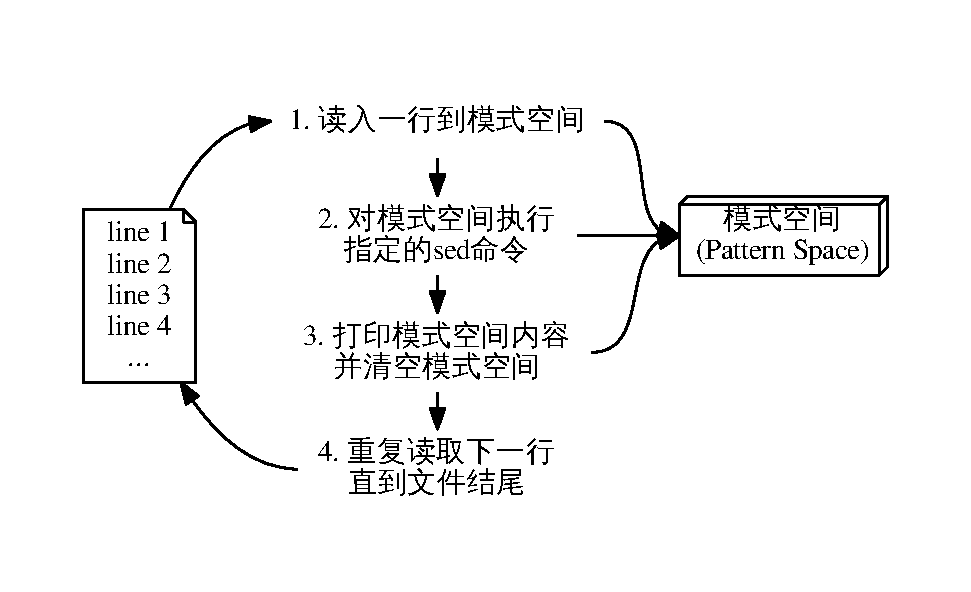
\includegraphics[width=.9\linewidth]{img/sed.pdf}
\end{itemize} % ends low level
\end{frame}
\begin{frame}[fragile]
\frametitle{运行sed}
\label{sec-2-1-2}
\begin{itemize}

\item sed options\ldots{} [script] [file]\ldots{}
\label{sec-2-1-2-1}%
\end{itemize} % ends low level
\begin{exampleblock}{常用选项}
\label{sec-2-1-2-2}


\begin{verbatim}
-n  安静模式,不打印模式空间内容
-e script 添加处理脚本
-f script-file 添加保存在文件中的脚本
-i 直接修改原始输入文件
\end{verbatim}
\end{exampleblock}
\begin{block}{注意}
\label{sec-2-1-2-3}

script内的命令可以用分号(;)或换行分隔
\end{block}
\end{frame}
\begin{frame}
\frametitle{sed工作原理}
\label{sec-2-1-3}
\begin{itemize}

\item sed按以下方式循环处理每一行(sed从前至后仅处理一遍):
\label{sec-2-1-3-1}%
\begin{enumerate}
\item 从输入流中读取一行,去掉尾部的换行符后放入模式空间
\item 执行脚本,脚本中的每条命令可以与一个地址关联,地址可认为是某种条件码,命令仅在条件满足时才被执行。
\item 当执行至脚本结尾时,除非指定了-n选项,否则模式空间的内容将被打印到输出流,并且如果前面被删除了换行符则将其添加回去,
\item 回到步骤1,开始下一次循环。
\end{enumerate}
\end{itemize} % ends low level
\begin{block}{注意}
\label{sec-2-1-3-2}

除非使用了类似D这样的特殊命令,每次循环的最后,模式空间都将被清空。
\end{block}
\end{frame}
\begin{frame}[fragile]
\frametitle{地址}
\label{sec-2-1-4}
\begin{exampleblock}{行选择}
\label{sec-2-1-4-1}


\begin{verbatim}
n 第n行
m~n 从第m行开始,每n行,如1~2表示所有奇数行
$ 末行
/regexp/ 与正则表达式regexp匹配的行
\%regexp% 同上,但把默认的/替换成其他字符,如%
\end{verbatim}
\end{exampleblock}
\begin{block}{范围选择}
\label{sec-2-1-4-2}


\begin{verbatim}
m,n 从第m行至第n行
n,/regexp/ 从第n行往后至与regexp匹配的第一行
/regexp1/,/regexp2/
m,n! 除m~n行外
/regexp/! 除与regexp匹配的行外
\end{verbatim}
\end{block}
\end{frame}
\begin{frame}
\frametitle{常用命令}
\label{sec-2-1-5}
\begin{itemize}

\item \#   注释
\label{sec-2-1-5-1}%

\item q    退出
\label{sec-2-1-5-2}%

\item d    删除模式空间,立即进入下一循环
\label{sec-2-1-5-3}%

\item p    打印模式空间
\label{sec-2-1-5-4}%

\item n    打印模式空间(若无-n选项),然后将其内容替换为下一行或者退出
\label{sec-2-1-5-5}%

\item \{ command1; command2; \ldots{} \}    命令组,命令之间用分号隔开
\label{sec-2-1-5-6}%
\end{itemize} % ends low level
\end{frame}
\begin{frame}[fragile]
\frametitle{sed简单示例}
\label{sec-2-1-6}
\begin{exampleblock}{示例}
\label{sec-2-1-6-1}


\begin{minted}[]{bash}
sed '' file
sed -n '' file
sed -n '1,$p' file
sed '10q' file
sed -n '$p' file
sed '/^$/d' file
sed '\|^#|d' file
sed -n 'n;p' file
sed -n -e 'n' -e 'p' file  #同上
sed '1~2d' file            #同上
sed '2~2!d' file           #同上
\end{minted}
\end{exampleblock}
\end{frame}
\begin{frame}[fragile]
\frametitle{s命令(搜索替换)}
\label{sec-2-1-7}
\begin{exampleblock}{示例}
\label{sec-2-1-7-1}


\begin{minted}[]{bash}
cat well.txt
Sam reads well, sam writes well, sam sings well.
sed 's/sam/tom/' well.txt
sed 's/sam/tom/i' well.txt
sed 's#sam#tom#gi' well.txt
sed 's|sam|tom|2i' well.txt
sed 's$sam$tom$2gi' well.txt
\end{minted}
\end{exampleblock}
\begin{block}{试一试}
\label{sec-2-1-7-2}


\begin{verbatim}
echo 'this costs 23, and that costs 35' >costs.txt
1. 在所有价格前面加上美元符$
2. 若把23改成.23,把35改成3.5,怎么加美元符$?
\end{verbatim}
\end{block}
\note{答案


\begin{minted}[]{bash}
sed 's/[0-9]\+/$&/g' costs.txt
sed 's/[0-9]*\.\?[0-9]\+/$&/g' costs.txt
sed 's/\([0-9]*\.\)\?[0-9]\+/$&/g' costs.txt
\end{minted}
}
\end{frame}
\begin{frame}[fragile]
\frametitle{a,i,c命令}
\label{sec-2-1-8}
\begin{exampleblock}{示例}
\label{sec-2-1-8-1}


\begin{minted}[]{bash}
sed '3a\
line 1\
line 2' file  #在第3行后追加(append)2行内容

sed '10i\
line 1\
line 2' file  #在第10行前插入(insert)2行内容

sed '/regex/c
line 1
line 2' file  #将与regex匹配的行修改(change)为2行内容
\end{minted}
\end{exampleblock}
\end{frame}
\begin{frame}[fragile]
\frametitle{r,w,y,=命令和-f选项}
\label{sec-2-1-9}
\begin{exampleblock}{示例}
\label{sec-2-1-9-1}


\begin{minted}[]{bash}
sed '3r file2' file1 #将file2的内容插入file1第3行之后
sed -n '/:\/\//w file2' file1 #匹配://的行号保存至file2
sed -n '\#://#w file2' file1  #同上
sed 'y/aeiou/xxxxx/' file #逐字符替换,前后长度需一致!
sed -n '$=' file          #打印最后一行的行号,即wc -l

cat sedscript             #准备好sed脚本文件
1,3d                      #每行包含一条sed命令
s/old/new/g
y/abc/xyz/
sed -n -f sedscript file  #利用-f让sed根据脚本处理file
\end{minted}
\end{exampleblock}
\end{frame}
\begin{frame}[fragile]
\frametitle{e命令}
\label{sec-2-1-10}
\begin{itemize}

\item 将sed处理得到的结果提交给shell执行。
\label{sec-2-1-10-1}%
\end{itemize} % ends low level
\begin{exampleblock}{示例}
\label{sec-2-1-10-2}


\begin{minted}[]{bash}
#复制目录结构
find teach/2014-linux/ -type d \
| sed 's/2014/2016/' \
| sed -n 's/^/mkdir -p /e'
\end{minted}
\end{exampleblock}
\end{frame}
\begin{frame}[fragile]
\frametitle{sed应用举例}
\label{sec-2-1-11}
\begin{itemize}

\item 实现basename命令\\
\label{sec-2-1-11-1}%
\begin{minted}[]{bash}
find /usr/bin -name 'mk*' -exec basename {} \;
\end{minted}

\item 实现dirname命令\\
\label{sec-2-1-11-2}%
\begin{minted}[]{bash}
find . -name '*.ppt' -exec dirname {} \; | sort | uniq
\end{minted}

\item 抽取网页文本内容
\label{sec-2-1-11-3}%

\item unix文本和windows文本转换
\label{sec-2-1-11-4}%
\end{itemize} % ends low level
\end{frame}
\begin{frame}
\frametitle{sed高级命令}
\label{sec-2-1-12}
\begin{itemize}

\item D\\
\label{sec-2-1-12-1}%
如果模式空间不含换行符,则与d相同。否则,删除模式空间内容至第一个换行符(包含该换行符),然后对模式空间重新执行一遍所有命令(不读入新行)。

\item N\\
\label{sec-2-1-12-2}%
为模式空间追加换行符和一新行,如果没有新行可读,则直接退出sed,不再执行后续命令。

\item P\\
\label{sec-2-1-12-3}%
打印模式空间内容至第一个换行符(包括该换行符)
\end{itemize} % ends low level
\end{frame}
\begin{frame}[fragile]
\frametitle{sed高级命令}
\label{sec-2-1-13}
\begin{exampleblock}{示例}
\label{sec-2-1-13-1}


\begin{minted}[]{bash}
sed -n 'N;D' students.db  #打印末行
sed -n 'N;P' students.db  #打印奇数行
sed -n '=' books.db | sed 'N;s/\n/ /'  #加行号
\end{minted}
\end{exampleblock}
\begin{block}{想一想:下面哪些命令可以打印出输入的最末2行?}
\label{sec-2-1-13-2}

\begin{enumerate}
\item sed `N;N;D' students.db
\item sed -n `\$-1,\$p' students.db
\item head -4 students.db | sed -n `N;\$p'
\item head -3 students.db | sed -n `N;\$p'
\item sed `N;\$!D' students.db
\end{enumerate}
\end{block}
\note{答案

\begin{enumerate}
\item 不能,因为每读2行,只删1行,因此累积下来最后会剩下约一半的行
\item 不能,因为sed只有处理到最后一行才知道这是末行,不能处理\$-1这种地址
\item 能,因为行数为偶数,N能读到末行(处理过程:读第1行,N追加第2行,清空,读第3行,N追加第4行,打印)
\item 不能,因为行数为奇数,N不能读到末行,直接退出,无输出(处理过程:读第1行,N追加第2行,清空,读第3行,N读不到新行,退出)
\item 正解(处理过程:读第1行,N追加第2行,D删除第1行后非空,返回N追加第3行,D删除第2行后非空,返回N追加第4行,\ldots{}...,返回N追加末行,此时不执行D操作,输出)
\end{enumerate}
}
\end{frame}
\begin{frame}
\frametitle{暂存空间(hold space)}
\label{sec-2-1-14}
\begin{itemize}

\item sed运行时可以使用两个缓存空间
\label{sec-2-1-14-1}%
\begin{itemize}

\item 模式空间(pattern space)
\label{sec-2-1-14-1-1}%

\item 暂存空间(hold space)
\label{sec-2-1-14-1-2}%
\end{itemize} % ends low level
\end{itemize} % ends low level
\begin{exampleblock}{模式空间}
\label{sec-2-1-14-2}

\begin{enumerate}
\item 不断从输入获取新行
\item 可对其内容执行sed命令
\item 一般每次执行完sed命令后会被清空
\end{enumerate}
\end{exampleblock}
\begin{block}{暂存空间}
\label{sec-2-1-14-3}

\begin{enumerate}
\item 默认无内容,但可以从模式空间获得内容
\item 不能直接对其内容执行sed命令
\item 不会自动清空其内容
\end{enumerate}
\end{block}
\end{frame}
\begin{frame}
\frametitle{在模式空间和暂存空间之间传递数据}
\label{sec-2-1-15}
\begin{itemize}

\item x -- exchange\\
\label{sec-2-1-15-1}%
交换模式空间和暂存空间的内容。

\item h -- hold pattern space\\
\label{sec-2-1-15-2}%
把模式空间的内容复制到暂存空间(覆盖)

\item H -- Hold pattern space\\
\label{sec-2-1-15-3}%
把模式空间的内容追加到暂存空间尾部(用换行符分隔)

\item g -- get contents of hold area\\
\label{sec-2-1-15-4}%
把暂存空间的内容复制到模式空间(覆盖)

\item G -- Get contents of hold area\\
\label{sec-2-1-15-5}%
把暂存空间的内容追加到模式空间尾部(用换行符分隔)
\end{itemize} % ends low level
\end{frame}
\begin{frame}[fragile]
\frametitle{暂存空间使用示例}
\label{sec-2-1-16}
\begin{exampleblock}{示例}
\label{sec-2-1-16-1}


\begin{minted}[]{bash}
#在行间加空行
sed 'G' students.db       #每行前加空行
sed 'x;p;x' students.db   #每行后加空行
#实现tac file命令
sed -n '1!G;$!h;$p' students.db
sed '1!G;$!h;$!d' students.db
\end{minted}
\end{exampleblock}
\end{frame}
\begin{frame}[fragile]
\frametitle{流程控制}
\label{sec-2-1-17}
\begin{exampleblock}{标签}
\label{sec-2-1-17-1}


\begin{verbatim}
:label    #设置标签
\end{verbatim}
\end{exampleblock}
\begin{block}{分支(branch)}
\label{sec-2-1-17-2}


\begin{verbatim}
b label   #跳转到标签位置
b         #跳转到脚本结尾
\end{verbatim}
\end{block}
\begin{exampleblock}{测试(test)}
\label{sec-2-1-17-3}


\begin{verbatim}
t label   #如果成功执行了s命令,则跳转到标签
t         #如果成功执行了s命令,则跳转到脚本结尾
\end{verbatim}
\end{exampleblock}
\end{frame}
\begin{frame}[fragile]
\frametitle{流程控制示例}
\label{sec-2-1-18}
\begin{exampleblock}{示例}
\label{sec-2-1-18-1}


\begin{minted}[]{bash}
sed ':a;N;6,$D;ba' students.db     #实现tail -5命令
sed ':m;s/^.\{1,79\}$/ &/;tm' students.db #实现文本右对齐
\end{minted}
\end{exampleblock}
\begin{block}{试一试}
\label{sec-2-1-18-2}

\begin{enumerate}
\item 如何实现文本居中对齐?
\item 如何在/usr/share/dict/words中搜索任意长度的回文单词?
\end{enumerate}
\end{block}
\note{答案

\begin{enumerate}
\item sed `:a;s/^.\{1,78\}\$/ \& \emph{;ta' students.db 2. sed -n `h;:b;s/^\(.\)\(.*\)\1\$}\2/;tb;/^.\?\$/\{g;p\}' /usr/share/dict/words
\end{enumerate}
}
\end{frame}
\subsection{awk}
\label{sec-2-2}
\begin{frame}
\frametitle{awk简介}
\label{sec-2-2-1}
\begin{itemize}

\item awk是由Al Aho,Peter Weinberger和Brian Kernighan 设计与实现的一种模式扫描与处理语言。
\label{sec-2-2-1-1}%

\item awk最早的设计目的是针对报表生成的一种小巧且具表达力的语言,awk对于处理格式化结构的文本文件特别强大。
\label{sec-2-2-1-2}%
\end{itemize} % ends low level
\end{frame}
\begin{frame}[fragile]
\frametitle{awk入门}
\label{sec-2-2-2}
\begin{itemize}

\item 引例\\
\label{sec-2-2-2-1}%
\begin{minted}[]{bash}
cat emp.data
Beth  4.00 0
Dan   3.75 0
Kathy 4.00 10
Mark  5.00 20
Mary  5.50 22
Susie 4.25 18
\end{minted}
注:第1列为员工姓名,第2列为时薪,第3列为工作时间

\begin{enumerate}
\item 要求打印出所有工作时间大于0的员工应发薪水
\end{enumerate}

\begin{minted}[]{bash}
awk '$3>0 {print $1, $2*$3}' emp.data
\end{minted}
\begin{enumerate}
\item 要求打印出工作时间为0的员工的姓名
\end{enumerate}

\begin{minted}[]{bash}
awk '$3==0 {print $1}' emp.data
\end{minted}
\end{itemize} % ends low level
\end{frame}
\begin{frame}[fragile]
\frametitle{awk工作原理}
\label{sec-2-2-3}
\begin{itemize}

\item awk程序结构
\label{sec-2-2-3-1}%
\begin{itemize}

\item 引例中位于引号内的部分就是awk程序,awk程序由如下形式的语句构成:\\
\label{sec-2-2-3-1-1}%
\begin{verbatim}
pattern {action}
pattern {action}
......
\end{verbatim}

\item awk程序依次扫描每行输入,每一行都会与每个pattern比较,若匹配则执行相应的action。
\label{sec-2-2-3-1-2}%
\end{itemize} % ends low level
\begin{exampleblock}{如果省略\{action\}部分,则打印与pattern匹配的整行}
\label{sec-2-2-3-1-3}


\begin{verbatim}
awk '$3==0' emp.data  #打印工作时间为0的员工的整条记录
\end{verbatim}
\end{exampleblock}
\begin{block}{如果省略pattern部分,则每一行都执行对应的action}
\label{sec-2-2-3-1-4}


\begin{verbatim}
awk '{print $1}' emp.data  #打印所有员工的姓名
\end{verbatim}
\end{block}
\end{itemize} % ends low level
\end{frame}
\begin{frame}[fragile]
\frametitle{运行awk程序}
\label{sec-2-2-4}
\begin{exampleblock}{方式1:awk `program' input files}
\label{sec-2-2-4-1}


\begin{minted}[]{bash}
awk '$3==0 {print $1}' file1 file2
\end{minted}
\end{exampleblock}
\begin{block}{方式2:awk `program'}
\label{sec-2-2-4-2}


\begin{minted}[]{bash}
awk '$3==0 {print $1}'  #输入来自标准输入
Beth  4.00 10
Kathy 3.58 0
Kathy
\end{minted}
\end{block}
\begin{exampleblock}{方式3:awk -f progfile input files}
\label{sec-2-2-4-3}


\begin{minted}[]{bash}
cat prog.awk
$3==0 {print $1}
awk -f prog.awk file1 file2
\end{minted}
\end{exampleblock}
\end{frame}
\begin{frame}[fragile]
\frametitle{字段(field)和内置变量}
\label{sec-2-2-5}
\begin{itemize}

\item awk默认每行为一条记录,记录内的字段分隔符为空格符或tab符
\label{sec-2-2-5-1}%

\item 特定字段:\$1,\$2,\ldots{}
\label{sec-2-2-5-2}%

\item 整条记录:\$0
\label{sec-2-2-5-3}%

\item 当前记录字段个数:NF
\label{sec-2-2-5-4}%

\item 当前记录最后一个字段:\$NF
\label{sec-2-2-5-5}%

\item 当前记录号:NR
\label{sec-2-2-5-6}%
\end{itemize} % ends low level
\begin{exampleblock}{示例}
\label{sec-2-2-5-7}


\begin{minted}[]{bash}
1. who | awk '{print NF,$1,$NF}'
2. awk '{print NR, $0}' emp.data
3. awk '{print "total pay for",$1,"is",$2*$3}' emp.data
\end{minted}
\end{exampleblock}
\end{frame}
\begin{frame}[fragile]
\frametitle{更好的输出}
\label{sec-2-2-6}
\begin{exampleblock}{示例}
\label{sec-2-2-6-1}


\begin{minted}[]{bash}
1. {printf("pay for %s is %2.2f\n", $1, $2*$3)}
2. {printf("%-8s $%6.2f\n", $1, $2*$3)}
3. awk '{printf("%6.2f  %s\n", $2*$3, $0)}' emp.data \
| sort
\end{minted}
\end{exampleblock}
\end{frame}
\begin{frame}[fragile]
\frametitle{模式}
\label{sec-2-2-7}
\begin{itemize}

\item 模式匹配结果为真,则执行相应动作\\
\label{sec-2-2-7-1}%
\begin{verbatim}
1. /regex/
2. !/regex/
3. $0~/regex/
4. $1!~/regex/
5. NF==0
6. NR%2!=0
7. (NR>5)&&(length($3)<30)
8. (NR==3),(NR==5)
9. /<[Hh][Tt][Mm][Ll]>/,/<\/[Hh][Tt][Mm][Ll]>/
10. 1
\end{verbatim}
\end{itemize} % ends low level
\end{frame}
\begin{frame}[fragile]
\frametitle{模式}
\label{sec-2-2-8}
\begin{exampleblock}{示例}
\label{sec-2-2-8-1}


\begin{minted}[]{bash}
$2 >= 5
$2*$3 > 50{printf("$%.2f for %s\n", $2*$3, $1)}
$1 == "Susie"
/Susie/
$2 >=4 || $3 >=20
!($2 <4 && $3 <20)
\end{minted}
\end{exampleblock}
\end{frame}
\begin{frame}[fragile]
\frametitle{BEGIN和END}
\label{sec-2-2-9}
\begin{itemize}

\item BEGIN模式所对应的动作在awk处理第一行之前执行
\label{sec-2-2-9-1}%

\item END模式所对应的动作在awk处理完末行之后执行
\label{sec-2-2-9-2}%
\end{itemize} % ends low level
\begin{exampleblock}{示例}
\label{sec-2-2-9-3}


\begin{minted}[]{bash}
BEGIN {print "NAME   RATE  HOURS"; print ""}
      {print}
  END {print "Total:", NR, "records"}
\end{minted}
\end{exampleblock}
\end{frame}
\begin{frame}[fragile]
\frametitle{计算}
\label{sec-2-2-10}
\begin{exampleblock}{示例}
\label{sec-2-2-10-1}


\begin{minted}[]{bash}
#计数:累计工作时间超过15小时的员工人数
$3>15 {emp = emp +1}
  END {print emp, "employees worked more than 15 hours"}

#统计:计算员工总工资和平均工资
    {pay += $2*$3}
END {print NR, "employees"
     print "total pay is", pay
     print "average pay is", pay/NR
    }
\end{minted}
\end{exampleblock}
\end{frame}
\begin{frame}[fragile]
\frametitle{处理文本}
\label{sec-2-2-11}
\begin{exampleblock}{示例}
\label{sec-2-2-11-1}


\begin{minted}[]{bash}
#打印时薪最高的员工姓名及其时薪
$2 > maxrate {maxrate = $2; maxemp = $1}
         END {print "highest pay rate:", maxemp, maxrate}

#字符串连接:紧凑打印所有员工姓名
    {names = names $1 " "}
END {print names}

#打印末行
    {last = $0}
END {print last}
\end{minted}
\end{exampleblock}
\end{frame}
\begin{frame}[fragile]
\frametitle{内置函数}
\label{sec-2-2-12}
\begin{exampleblock}{示例}
\label{sec-2-2-12-1}


\begin{minted}[]{bash}
#打印每个员工的姓名长度
{print $1, length($1)}

#统计行数、单词数和字符数
    {nc += length($0) + 1
     nw += NF
    }
END {print NR,"lines,",nw,"words,",nc,"chars"}
\end{minted}
\end{exampleblock}
\end{frame}
\begin{frame}
\frametitle{内置函数(部分数值函数)}
\label{sec-2-2-13}


\begin{center}
\begin{tabular}{ll}
 函数名      &  返回值                  \\
\hline
 atan2(y,x)  &  y/x(-pi到pi)的反正切    \\
 cos(x)      &  x的余弦,x为弧度值      \\
 exp(x)      &  e的x次幂                \\
 int(x)      &  x向0取整                \\
 log(x)      &  求x的自然对数(以e为底)  \\
 rand()      &  [0,1)之间的随机数       \\
 sin(x)      &  x的正弦,x为弧度值      \\
 sqrt(x)     &  x的平方根               \\
 srand(x)    &  x为rand()的新随机种子   \\
\end{tabular}
\end{center}
\end{frame}
\begin{frame}[fragile]
\frametitle{数值函数使用举例}
\label{sec-2-2-14}
\begin{exampleblock}{示例}
\label{sec-2-2-14-1}


\begin{minted}[]{bash}
1. randint = int(n*rand())+1 #获得1到n之间的随机整数
2. x=int(x+0.5)  #四舍五入取整
3. awk 'BEGIN{cos(60*3.1415926/180)}'
4. echo 1000 | awk '{print log($1)/log(10)}'
\end{minted}
\end{exampleblock}
\end{frame}
\begin{frame}
\frametitle{内置函数(部分字符串函数)}
\label{sec-2-2-15}


\begin{center}
\begin{tabular}{ll}
 函数名             &  函数描述                                     \\
\hline
 gsub(r,s[,t])      &  在\$0/t中将r全局替换为s,返回替换次数         \\
 index(s,t)         &  返回t在s中首次出现的位置,返回0表示未找到    \\
 length(s)          &  返回s的长度                                  \\
 match(s,r)         &  测试s是否包含r,返回index或0                 \\
 split(s,a[,fs])    &  将s拆分为数组a,分隔符为FS/fs,返回字段个数  \\
 sprintf(fmt,list)  &  返回按指定格式控制的字符串                   \\
 sub(r,s[,t])       &  类似于gsub(r,s[,t]),但仅替换1次             \\
 substr(s,p[,n])    &  返回s从位置p开始[的长度为n]的子串            \\
\end{tabular}
\end{center}
\end{frame}
\begin{frame}[fragile]
\frametitle{字符串函数使用举例}
\label{sec-2-2-16}
\begin{exampleblock}{示例}
\label{sec-2-2-16-1}


\begin{minted}[]{bash}
1. awk 'BEGIN{print index("banana","an")}'
2. echo banana | awk '{gsub(/an/,"ok");print}'
3. echo banana | awk '{sub(/an/,"&d&");print}'
4. echo banana | awk '{print substr($1,2,2)}'
5. echo banana | awk '{print substr($1,3)}'
6. echo '10/01/2016' \
| awk '{split($0,date,"/");print date[3]}'
\end{minted}
\end{exampleblock}
\end{frame}
\begin{frame}[fragile]
\frametitle{自定义函数}
\label{sec-2-2-17}
\begin{exampleblock}{示例}
\label{sec-2-2-17-1}


\begin{minted}[]{bash}
{ print max($1, max($2,$3)) }
function max(m,n){
  return m>n ? m : n
}
\end{minted}
\end{exampleblock}
\end{frame}
\begin{frame}[fragile]
\frametitle{控制流语句}
\label{sec-2-2-18}
\begin{itemize}

\item if-else
\label{sec-2-2-18-1}%
\end{itemize} % ends low level
\begin{exampleblock}{示例}
\label{sec-2-2-18-2}


\begin{minted}[]{bash}
$2 > 6 {n++; pay += $2*$3}
END    { if (n>0)
             print n, "employees, total pay is",pay,
                      "average pay is",pay/n
         else
             print "no employees are paid more than $6/h"
       }
\end{minted}
\end{exampleblock}
\end{frame}
\begin{frame}[fragile]
\frametitle{控制流语句}
\label{sec-2-2-19}
\begin{itemize}

\item while
\label{sec-2-2-19-1}%
\end{itemize} % ends low level
\begin{exampleblock}{示例:计算银行复利}
\label{sec-2-2-19-2}


\begin{minted}[]{bash}
# interest1 - compute compound interest
#  input: amount rate years
# output: compounded value at the end of each year
{ i=1
  while (i <= $3) {
    printf("\t%.2f\n", $1*(1+$2)^i)
    i++
  }
}

awk -f interest1
1000 .06 5
\end{minted}
\end{exampleblock}
\end{frame}
\begin{frame}[fragile]
\frametitle{控制流语句}
\label{sec-2-2-20}
\begin{itemize}

\item for
\label{sec-2-2-20-1}%
\end{itemize} % ends low level
\begin{exampleblock}{示例}
\label{sec-2-2-20-2}


\begin{minted}[]{bash}
# interest2 - compute compound interest
#  input: amount rate years
# output: compounded value at the end of each year
{ for (i=1; i<=$3; i++)
    printf("\t%.2f\n", $1*(1+$2)^i)
}
\end{minted}
\end{exampleblock}
\end{frame}
\begin{frame}[fragile]
\frametitle{控制流语句应用举例}
\label{sec-2-2-21}
\begin{exampleblock}{示例:查找相邻重复词(包括行首与前一行末的重复)}
\label{sec-2-2-21-1}


\begin{minted}[]{bash}
cat double
NF>0 {
if ($1 == lastword)
  printf “%s\t%d: %s\n”, FILENAME, FNR, $1
for ( i=1;i<NF;i++ )
  if ( $i == $(i+1) )
    printf “%s\t%d: %s\n”, FILENAME, FNR, $i
lastword = $NF
}

awk -f double file1 file2 file3
\end{minted}
\end{exampleblock}
\end{frame}
\begin{frame}[fragile]
\frametitle{数组}
\label{sec-2-2-22}
\begin{exampleblock}{示例}
\label{sec-2-2-22-1}


\begin{minted}[]{bash}
#反向输出每一行(类似tac命令)   while版
    { line[NR] = $0 }
END { i = NR
      while (i>0) {
        print line[i]
        i--
      } 
    }
#反向输出每一行(类似tac命令)   for版
    { line[NR] = $0 }
END { for (i=NR; i>0; i--)
        print line[i]
    }
\end{minted}
\end{exampleblock}
\end{frame}
\begin{frame}[fragile]
\frametitle{其他简单示例}
\label{sec-2-2-23}
\begin{exampleblock}{awk简单程序示例}
\label{sec-2-2-23-1}


\begin{minted}[]{bash}
1. END {print NR} #打印行数
2. NR==10         #打印第10行
3. {print $NF}    #打印每行最后一个字段
4. {field=$NF}END{print field} #打印末行末字段
5. NF>4  #打印多于4个字段的行
6. $NF>4 #打印最后一个字段的值大于4的行
7. {nf=nf+NF}END{print nf} #打印所有行字段个数之和
8. /Beth/{n++}END{print n} #打印包含Beth的行数
9. $1>max{max=$1;maxline=$0}END{print max,maxline}
10. NF>0
11. length($0) > 80
12. {print NF, $0}
\end{minted}
\end{exampleblock}
\end{frame}
\begin{frame}[fragile]
\frametitle{其他简单示例}
\label{sec-2-2-24}
\begin{exampleblock}{awk简单程序示例(2)}
\label{sec-2-2-24-1}


\begin{minted}[]{bash}
13. {print $2, $1}
14. {temp=$1;$1=$2;$2=temp;print}
15. {$1=NR;print}
16. {$2="";print}
17. {for(i=NF;i>0;i--)printf("%s ", $i)
 printf("\n")
}
18. {sum = 0
 for (i=1;i<=NF;i++) sum+=$i
 print sum
}
19. {for(i=1;i<=NF;i++)sum+=$i}END{print sum}
20. {for(i=1;i<=NF;i++)if($i<0)$i=-$i}print}
\end{minted}
\end{exampleblock}
\end{frame}
\begin{frame}[fragile]
\frametitle{指定字段分隔符}
\label{sec-2-2-25}
\begin{exampleblock}{方法1:-F选项}
\label{sec-2-2-25-1}


\begin{minted}[]{bash}
awk -F: '/bash/{print $1,$2}' /etc/passwd
\end{minted}
\end{exampleblock}
\begin{block}{方法2:在BEGIN中为FS内置变量赋值}
\label{sec-2-2-25-2}


\begin{minted}[]{bash}
BEGIN  {FS=':'}
/bash/ {print $1,$2}
\end{minted}
\end{block}
\end{frame}
\begin{frame}
\frametitle{awk内置变量}
\label{sec-2-2-26}


\begin{center}
\begin{tabular}{ll}
 变量名    &  含义                                   \\
\hline
 FILENAME  &  当前文件名                             \\
 FS        &  输入的字段分隔符(默认为空格符和tab符)  \\
 RS        &  输入的记录分隔符(默认为换行符)         \\
 NF        &  当前记录字段个数                       \\
 NR        &  当前记录的序号                         \\
 FNR       &  当前文件的当前记录号                   \\
 OFMT      &  数字的输出格式(默认为\%.6g)            \\
 OFS       &  输出的字段分隔符(默认为空格符)         \\
 ORS       &  输出的记录分隔符(默认为换行符)         \\
\end{tabular}
\end{center}
\end{frame}
\begin{frame}[fragile]
\frametitle{awk内置变量使用举例}
\label{sec-2-2-27}
\begin{exampleblock}{示例}
\label{sec-2-2-27-1}


\begin{verbatim}
cat stu.db
tom
19
male

mary
18
female
请将stu.db的内容转换为如下格式:
tom:19:male
mary:18:female
\end{verbatim}
\end{exampleblock}
\note{答案


\begin{minted}[]{bash}
awk 'BEGIN{FS="\n";RS="\n\n";OFS=":"}{print $1,$2,$3}' stu.db
\end{minted}
}
\end{frame}
\begin{frame}[fragile]
\frametitle{关联数组}
\label{sec-2-2-28}
\begin{itemize}

\item 问题:现有客户订货记录order.db如下:\\
\label{sec-2-2-28-1}%
\begin{verbatim}
cat order.db
Susie 400
John 100
Mary 200
Mary 300
John 100
Susie 100
Mary 100
John 200
Mary 600
Susie 500
\end{verbatim}
请统计每位客户的订货总数。
\end{itemize} % ends low level
\end{frame}
\begin{frame}[fragile]
\frametitle{关联数组}
\label{sec-2-2-29}
\begin{exampleblock}{统计每位客户的订货总数}
\label{sec-2-2-29-1}


\begin{minted}[]{bash}
awk '{sum[$1]+=$2}
  END{for(u in sum)print n,sum[n]}' order.db
\end{minted}
\end{exampleblock}
\begin{block}{试一试}
\label{sec-2-2-29-2}

请用awk进行词频统计,并打印出每个单词出现的次数。
\end{block}
\note{答案


\begin{minted}[]{bash}
cat >wc.awk
{gsub(/[[:punct:]]/,"")
 for (i=1; i<=NF; i++)
   dict[$i]++
}
END{for (w in dict)
      print w, dict[w] | "sort -k2 -rn"
}

tr 'A-Z' 'a-z' <students | awk -f wc.awk
\end{minted}
}
\end{frame}
\begin{frame}[fragile]
\frametitle{综合实例}
\label{sec-2-2-30}
\begin{itemize}

\item 问题:现有学生成绩清单score.list如下:\\
\label{sec-2-2-30-1}%
\begin{verbatim}
jasper: 80 82 84 84 88 92
andrea: 85 89 90 90 94 95
ellis: 89 90 92 96 96 98
mona: 70 70 77 83 85 89
john: 78 85 88 91 92 94
dunce: 60 60 61 62 64 80

请统计:
(1)每位同学的平均分及等级(A,B,C,D,F)
(2)班平均成绩
(3)平均成绩高于或等与班平均的人数
(4)平均成绩低于班平均的人数
(5)每个等级的人数
\end{verbatim}
\end{itemize} % ends low level
\end{frame}
\begin{frame}[fragile]
\frametitle{综合实例}
\label{sec-2-2-31}


\begin{minted}[]{bash}
grep -v '^ *#' grade.awk
BEGIN { OFS = "\t" }
{ 
        total = 0
        for (i = 2; i <= NF; ++i)
          total += $i 
        avg = total / (NF - 1)
        student_avg[NR] = avg
        if (avg >= 90)  grade = "A"
        else if (avg >= 80) grade = "B"
        else if (avg >= 70) grade = "C"
        else if (avg >= 60) grade = "D"
        else grade = "F"        
        ++class_grade[grade]
        print $1, avg, grade 
}
\end{minted}
\end{frame}
\begin{frame}[fragile]
\frametitle{综合实例}
\label{sec-2-2-32}


\begin{minted}[]{bash}
END {
for (x = 1; x <= NR; x++)
        class_avg_total += student_avg[x]
class_average = class_avg_total / NR
for (x = 1; x <= NR; x++)
        if (student_avg[x] >= class_average)
          ++above_average
        else
          ++below_average
print ""
print "Class Average: ", class_average
print "At or Above Average: ", above_average
print "Below Average: ", below_average     
for (letter_grade in class_grade)
        print letter_grade ":", class_grade[letter_grade] \
  | "sort" }
\end{minted}
\end{frame}
\begin{frame}[fragile]
\frametitle{综合实例}
\label{sec-2-2-33}
\begin{itemize}

\item awk -f grade.awk score.list的输出结果如下:\\
\label{sec-2-2-33-1}%
\begin{verbatim}
jasper: 85      B
andrea: 90.5    A
ellis:  93.5    A
mona:   79      C
john:   88      B
dunce:  64.5    D

Class Average:  83.4167
At or Above Average:    4
Below Average:  2
A:      2
B:      2
C:      1
D:      1
\end{verbatim}
\end{itemize} % ends low level
\end{frame}

\end{document}
